\documentclass{beamer}

\mode<presentation> {
\usetheme{Warsaw}
\usecolortheme{seahorse}
}

\usepackage{subcaption}
\usepackage{tcolorbox}
\tcbuselibrary{skins}
\usepackage[table]{xcolor}
\usepackage{colortbl}
\usepackage{array, multirow, multicol, tabularx}
\usepackage{booktabs}
\usepackage{amsfonts}
\usepackage{amsmath}
\usepackage{amssymb}
\usepackage{setspace}
\usepackage{caption}
\usepackage{ragged2e}
\usepackage{bm}
\usefonttheme[onlymath]{serif}
\usepackage{amsthm}
\usepackage{textcomp}
\usepackage{graphicx}
\usepackage{tikz}
\usepackage{pifont}
\usetikzlibrary{shapes, positioning, calc, arrows.meta}
\usepackage{pgfplots}
\pgfplotsset{compat=1.18}
\usepackage[outline]{contour}
\setbeamertemplate{caption}[numbered]

% Colors (same values as the paper)
\definecolor{morado}{rgb}{.88,.50,.90}
\definecolor{darkgreen}{rgb}{0,0.39,0}
\definecolor{matlabBlue}{rgb}{0.000,0.380,0.900}

% Modern palette for the motivation schematic
\definecolor{primaryblue}{RGB}{37, 99, 235}
\definecolor{darkslate}{RGB}{15, 23, 42}
\definecolor{crimsonred}{RGB}{220, 38, 38}
\definecolor{forestgreen}{RGB}{22, 163, 74}
\definecolor{lightgraybg}{RGB}{248, 250, 252}
\definecolor{amberbg}{RGB}{217, 119, 6}

% Swatches for figure legends (same as the paper)
\DeclareRobustCommand{\legsolid}[1]{\textcolor{#1}{\rule[0.55ex]{1.6em}{0.8pt}}}
\DeclareRobustCommand{\legdotted}[1]{\textcolor{#1}{\makebox[1.6em][l]{\dotfill}}}

% Reference line at the bottom of a slide
\newcommand{\slideref}[1]{\vfill{\tiny #1}}

% Make the Warsaw head/foot slimmer (keep them visible, but reduce height)
\setbeamertemplate{headline}{%
  \leavevmode%
  \hbox{%
    \begin{beamercolorbox}[wd=\paperwidth,ht=2.1ex,dp=0.9ex]{section in head/foot}%
      \scriptsize\insertnavigation{\paperwidth}%
    \end{beamercolorbox}%
  }%
}

\setbeamertemplate{footline}{%
  \leavevmode%
  \hbox{%
    \begin{beamercolorbox}[wd=.50\paperwidth,ht=2.1ex,dp=0.9ex,left]{author in head/foot}%
      \scriptsize\hspace*{1ex}\insertshortauthor
    \end{beamercolorbox}%
    \begin{beamercolorbox}[wd=.40\paperwidth,ht=2.1ex,dp=0.9ex,center]{title in head/foot}%
      \scriptsize\insertshorttitle
    \end{beamercolorbox}%
    \begin{beamercolorbox}[wd=.10\paperwidth,ht=2.1ex,dp=0.9ex,right]{date in head/foot}%
      \scriptsize\insertframenumber/\inserttotalframenumber\hspace*{1ex}
    \end{beamercolorbox}%
  }%
  \vskip0pt%
}

\title[{October 26-28, 2026 CDMX, México}]{Neuromorphic Modeling and Control for a Coaxial Hexarotor UAV using Spiking Neural Networks}
\author[{XXVIII Congreso Mexicano de Robótica}]
{
    \texorpdfstring{
    \\ \textbf{Anel Olivares}, Gandhi Torres, Victor J. Silva\\ Eduardo S. Espinoza, Juan M. Bustamante, and Patricio Ordaz \\
    \vspace{0.15cm}
    \begin{center}
        \includegraphics[scale = .2]{images_comrob/Comrob_logo.png}
    \end{center}
   }
   { }
}
\date[October 2026]{}

% Recurrent population drawn inside a tikzpicture (used on the per-DOF slide):
% #1 node name, #2 position, #3 state symbol, #4 recurrent-function label
\newcommand{\popn}[4]{%
  \node[pop] (#1) at #2 {};
  \foreach \a/\r in {90/0.22, 210/0.22, 330/0.22, 30/0.12, 150/0.12, 270/0.12}
    \fill[primaryblue] ($(#1)+(\a:\r)$) circle (1.2pt);
  \draw[arr, color=primaryblue] (#1.north east) .. controls +(0.45,0.55) and +(-0.45,0.55) .. (#1.north west)
    node[pos=0.5, above, font=\tiny, text=primaryblue, inner sep=1pt] {#4};
}

% Cascade diagram at width #1 with the "Coaxial Hexarotor UAV" text replaced by the T6 figure.
% Plant block measured on a 200-dpi render of cascade_classic.pdf (1953 x 784 px):
% border x = 1698..1852, y = 96..628 px; original text at y = 326..400 px.
\newcommand{\cascadeTsix}[1]{%
\begin{tikzpicture}
  \node[inner sep=0, anchor=south west] (casc) at (0,0)
       {\includegraphics[width=#1]{images_hexa/cascade_classic.pdf}};
  \begin{scope}[x={(casc.south east)}, y={(casc.north west)}]
    \fill[white] (0.8735,0.4745) rectangle (0.9447,0.6020);
    \node[inner sep=0] at (0.9089,0.5383)
         {\includegraphics[width=\dimexpr #1*686/10000\relax]{images_hexa/dinamica_hexa3.pdf}};
  \end{scope}
\end{tikzpicture}}

\begin{document}
\contourlength{0.01cm}

\begin{frame}
    \titlepage
\end{frame}

\begin{frame}
    \frametitle{Content}
    \vspace{-0.2cm}
    \begin{columns}[T,onlytextwidth]
    \column{0.5\textwidth}\footnotesize\tableofcontents[sections={1-3}]
    \column{0.5\textwidth}\footnotesize\tableofcontents[sections={4-6}]
    \end{columns}
\end{frame}

%===================================================================
\section[Introduction]{Introduction}

\subsection{Problem statement}

%------------------------------------------------
% ============================================================
% Motivation — Von Neumann vs. Neuromorphic Computing
% ============================================================
\begin{frame}{Why Neuromorphic Computing?}

% Subtitle
\begin{center}
{\small\color{gray!80!black}\textbf{Rethinking how intelligent machines compute}}
\end{center}

\vspace{-0.2cm}

\centering
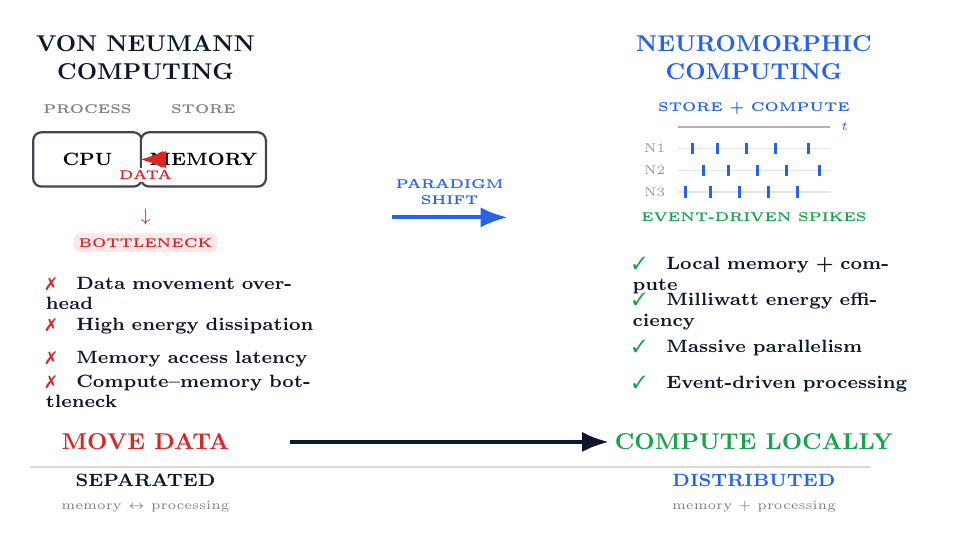
\begin{tikzpicture}[
    font=\scriptsize,
    scale=0.92,
    transform shape,
    >=Latex,
    cpubox/.style={
        draw=darkslate!80,
        fill=white,
        rounded corners=3pt,
        minimum width=1.5cm,
        minimum height=0.75cm,
        line width=0.8pt,
        font=\bfseries\scriptsize
    },
    cardbox/.style={
        draw=gray!30,
        fill=lightgraybg,
        rounded corners=6pt,
        line width=0.8pt
    }
]

% ============================================================
% HEADERS
% ============================================================
\node[font=\bfseries\small, align=center, text=darkslate] at (-4.2, 2.8) {VON NEUMANN\\COMPUTING};
\node[font=\bfseries\small, align=center, text=primaryblue] at (4.2, 2.8) {NEUROMORPHIC\\COMPUTING};

% ============================================================
% LEFT — VON NEUMANN
% ============================================================
\node[font=\tiny\bfseries, text=gray] at (-5.0, 2.1) {PROCESS};
\node[font=\tiny\bfseries, text=gray] at (-3.4, 2.1) {STORE};

\node[cpubox] (cpu) at (-5.0, 1.4) {CPU};
\node[cpubox] (memory) at (-3.4, 1.4) {MEMORY};

% Heavy data movement arrow
\draw[<->, line width=1.2pt, color=crimsonred] (cpu.east) -- (memory.west);
\node[font=\tiny\bfseries, text=crimsonred, fill=white, inner sep=1pt] at (-4.2, 1.18) {DATA};

% Bottleneck callout
\node[font=\scriptsize\bfseries, text=crimsonred] at (-4.2, 0.6) {$\downarrow$};
\node[font=\tiny\bfseries, fill=crimsonred!10, text=crimsonred, rounded corners=2pt, inner sep=2pt] at (-4.2, 0.25) {BOTTLENECK};

% Problems list
\node[anchor=west, text width=3.8cm] at (-5.7,-0.45) {\color{crimsonred}\ding{55}\quad \textbf{\color{darkslate}Data movement overhead}};
\node[anchor=west, text width=3.8cm] at (-5.7,-0.90) {\color{crimsonred}\ding{55}\quad \textbf{\color{darkslate}High energy dissipation}};
\node[anchor=west, text width=3.8cm] at (-5.7,-1.35) {\color{crimsonred}\ding{55}\quad \textbf{\color{darkslate}Memory access latency}};
\node[anchor=west, text width=3.8cm] at (-5.7,-1.80) {\color{crimsonred}\ding{55}\quad \textbf{\color{darkslate}Compute--memory bottleneck}};

% ============================================================
% CENTER — PARADIGM SHIFT
% ============================================================
\draw[->, line width=1.5pt, color=primaryblue] (-0.8, 0.6) -- (0.8, 0.6);
\node[font=\tiny\bfseries, text=primaryblue, align=center] at (0, 0.95) {PARADIGM\\SHIFT};

% ============================================================
% RIGHT — NEUROMORPHIC COMPUTING
% ============================================================
\node[font=\tiny\bfseries, text=primaryblue] at (4.2, 2.1) {STORE + COMPUTE};

% Spiking raster plot
\draw[gray!60, line width=0.6pt] (3.15, 1.85) -- (5.25, 1.85);
\node[font=\tiny, text=primaryblue, anchor=west] at (5.28, 1.85) {$t$};

\foreach \y/\lab in {1.55/N1, 1.25/N2, 0.95/N3}{
    \node[font=\tiny, text=gray!80, anchor=east] at (3.10,\y) {\lab};
    \draw[gray!20, line width=0.4pt] (3.15,\y) -- (5.25,\y);
}

% Spike ticks
\foreach \x in {3.35, 3.70, 4.10, 4.50, 4.95}{
    \draw[line width=1.0pt, color=primaryblue] (\x,1.55-0.08) -- (\x,1.55+0.08);
}
\foreach \x in {3.50, 3.85, 4.25, 4.65, 5.10}{
    \draw[line width=1.0pt, color=primaryblue] (\x,1.25-0.08) -- (\x,1.25+0.08);
}
\foreach \x in {3.25, 3.60, 4.00, 4.40, 4.80}{
    \draw[line width=1.0pt, color=primaryblue] (\x,0.95-0.08) -- (\x,0.95+0.08);
}

\node[font=\tiny\bfseries, text=forestgreen] at (4.2, 0.6) {EVENT-DRIVEN SPIKES};

% Advantages list
\node[anchor=west, text width=4.0cm] at (2.4,-0.20) {\color{forestgreen}\ding{51}\quad \textbf{\color{darkslate}Local memory + compute}};
\node[anchor=west, text width=4.0cm] at (2.4,-0.70) {\color{forestgreen}\ding{51}\quad \textbf{\color{darkslate}Milliwatt energy efficiency}};
\node[anchor=west, text width=4.0cm] at (2.4,-1.20) {\color{forestgreen}\ding{51}\quad \textbf{\color{darkslate}Massive parallelism}};
\node[anchor=west, text width=4.0cm] at (2.4,-1.70) {\color{forestgreen}\ding{51}\quad \textbf{\color{darkslate}Event-driven processing}};

% ============================================================
% MAIN TAKEAWAY BANNER
% ============================================================
\node[font=\small\bfseries, text=crimsonred] at (-4.2, -2.5) {MOVE DATA};
\draw[->, line width=1.5pt, color=darkslate] (-2.2, -2.5) -- (2.2, -2.5);
\node[font=\small\bfseries, text=forestgreen] at (4.2, -2.5) {COMPUTE LOCALLY};

% ============================================================
% BOTTOM ARCHITECTURAL CONTRAST
% ============================================================
\draw[gray!30, line width=0.6pt] (-5.8, -2.85) -- (5.8, -2.85);

\node[align=center, font=\scriptsize] at (-4.2, -3.2) {
    \textbf{\color{darkslate}SEPARATED}\\[1pt]
    {\tiny\color{gray}memory $\leftrightarrow$ processing}
};

\node[align=center, font=\scriptsize] at (4.2, -3.2) {
    \textbf{\color{primaryblue}DISTRIBUTED}\\[1pt]
    {\tiny\color{gray}memory + processing}
};

\end{tikzpicture}

\end{frame}

%------------------------------------------------
\begin{frame}{State of the art and gap}
\footnotesize
\begin{itemize}
    \item NEF-based SNN controllers have been used on underactuated systems and quadrotor UAVs\textsuperscript{1,2}.
    \item Neuromorphic control on Intel Loihi for a robotic arm\textsuperscript{3}.
    \item SNN flight control on neuromorphic hardware is limited to reduced-order cases: 1-DOF attitude\textsuperscript{4} and single-axis vertical landing\textsuperscript{5}.
\end{itemize}

\begin{table}[h]
    \centering
    \begin{tcolorbox}[
        tabularx = {l | X},
        title = Gap:,
        colback = primaryblue!8,
        colframe = primaryblue,
        fontupper=\footnotesize
    ]
        $\star$ & In these works the vehicle dynamics are simulated \textbf{outside} the neural framework.\\
        $\star$ & A fully neuromorphic architecture (dynamics \textbf{and} cascade controller in the NEF) has received little attention, especially beyond the quadrotor.\\
    \end{tcolorbox}
\end{table}

\slideref{[1] O. A. Garcia \emph{et al.}, CCE 2023. \quad [2] A. Olivares \emph{et al.}, IFAC-PapersOnLine, 2025; Neural Comput.\ Appl., 2026. \quad [3] T. DeWolf \emph{et al.}, Neuromorph.\ Comput.\ Eng., 2023. \quad [4] R. K. Stagsted \emph{et al.}, IROS 2020. \quad [5] J. Dupeyroux \emph{et al.}, ICRA 2021.}
\end{frame}

%------------------------------------------------

%------------------------------------------------
\begin{frame}{Problem and Contributions}

\centering
\vspace{-0.45cm}

{\scriptsize\bfseries\color{primaryblue}RESEARCH QUESTION\par}
\vspace{0.08cm}

{\normalsize\color{darkslate}
\parbox{0.96\linewidth}{\centering
Can the \textbf{\color{primaryblue}full flight stack} of a \textbf{coaxial hexarotor}
be realized inside a \textbf{\color{primaryblue}spiking SNN} without degrading
closed-loop tracking?}\par}

\vspace{0.18cm}

{\scriptsize\bfseries\color{primaryblue}CONTRIBUTIONS\par}
\vspace{0.06cm}

{\small
\begin{itemize}\setlength\itemsep{4pt}
    \item[\textcolor{primaryblue}{\ding{51}}] \textbf{Full stack in NEF/Nengo}: model + cascade control realized as a spiking network.
    \item[\textcolor{primaryblue}{\ding{51}}] \textbf{Validation}: trajectory tracking vs. MATLAB/Simulink baseline.
    \item[\textcolor{primaryblue}{\ding{51}}] \textbf{Modularity}: decoupled control modules across UAV subsystems.
\end{itemize}
}

\end{frame}

%===================================================================
\section[Platform]{Hexarotor and cascade control}
\subsection{T6 coaxial hexarotor}
%------------------------------------------------
% Visual separator slide (T6 coaxial figure only)
\begin{frame}{T6 coaxial hexarotor}
\centering
\includegraphics[width=\linewidth,height=0.78\textheight,keepaspectratio]{images_hexa/dinamica_hexa3.pdf}
\end{frame}

\subsection{Conventional cascade control}
%------------------------------------------------
% Cascade scheme at full paper width; the "Coaxial Hexarotor UAV" text inside the plant block
% is covered and replaced by a small T6 figure (block border and arrows untouched).
% Block measured on the 200-dpi render of cascade_classic.pdf (1953 x 784 px):
% border x = 1698..1852, y = 96..628 px; original text at y = 326..400 px.
\begin{frame}{Cascade control scheme}
\vspace{-0.35cm}
\makebox[\linewidth][c]{\cascadeTsix{\paperwidth}}
\end{frame}

%===================================================================
\section[Modeling]{Neuromorphic modeling}

\subsection{Six second-order subsystems}
\begin{frame}{From rigid body to six subsystems}
\centering
\small
$\dot{\bm{\xi}} = \bm{V},\quad m\dot{\bm{V}} = \bm{R}\bm{F},\quad
\mathbb{I}\dot{\bm{\Omega}} = -\bm{\Omega}\times\mathbb{I}\bm{\Omega}+\bm{\Gamma}$

\vspace{0.08cm}
{\footnotesize $u=\textstyle\sum_{i=1}^{6} f_i,\qquad \bm{\Gamma}=\bm{\Gamma}(f_i,\gamma_i)$ \ (three coaxial pairs)}

\vspace{0.25cm}
{\color{primaryblue}$\big\downarrow$}\ {\footnotesize near hover, $\psi\approx 0$}

\vspace{0.2cm}
\begin{tcolorbox}[colback=primaryblue!6, colframe=primaryblue, width=0.86\linewidth,
                  title={\centering Every degree of freedom:\quad $\ddot\zeta=\upsilon_\zeta$}]
\centering
\renewcommand{\arraystretch}{1.55}
\begin{tabular}{l|l||l|l}
$\zeta$ & $\upsilon_\zeta$ & $\zeta$ & $\upsilon_\zeta$\\ \hline
$z$ & $-\dfrac{u}{m}\cos\theta\cos\phi+g$ & $\theta$ & $\Gamma_\theta/I_{yy}$\\
$x$ & $-g\tan\theta$                       & $\phi$   & $\Gamma_\phi/I_{xx}$\\
$y$ & $g\tan\phi/\cos\theta$               & $\psi$   & $\Gamma_\psi/I_{zz}$\\
\end{tabular}
\end{tcolorbox}

\vspace{0.1cm}
{\scriptsize\color{gray} Altitude, longitudinal $(x,\theta)$, lateral $(y,\phi)$ and directional $(\psi)$ subsystems.
Aerodynamics, wind and actuator dynamics neglected.}
\end{frame}

\subsection{Recurrent spiking populations}
\begin{frame}{Each subsystem as a recurrent spiking population}
\begin{columns}[c]
\column{0.50\textwidth}
\centering
\includegraphics[width=\linewidth]{images_hexa/NLS_population.pdf}

{\scriptsize $h(t)=\tfrac{1}{\tau}e^{-t/\tau}$ \ (synaptic filter)}

\column{0.50\textwidth}
\small
Target:\quad $\dot\chi = F(\chi)+G(\upsilon)$

\vspace{0.1cm}
NEF (3rd principle):
\begin{tcolorbox}[colback=morado!10, colframe=morado!80, left=1mm, right=1mm, top=0.5mm, bottom=0.5mm]
\centering
$F'(\chi)=\tau F(\chi)+\chi$\\[2pt] $G'(\upsilon)=\tau G(\upsilon)$
\end{tcolorbox}
For $\chi=[\zeta,\ \dot\zeta]^\top$:
\[
F'_\zeta=\begin{bmatrix}\chi_1+\tau\chi_2\\ \chi_2\end{bmatrix},\qquad
G'_\zeta=\tau\begin{bmatrix}0\\ \upsilon_\zeta\end{bmatrix}
\]
\begin{center}
\colorbox{primaryblue!8}{\parbox{0.92\linewidth}{\centering\footnotesize
\textbf{One template, six populations} --- only $\upsilon_\zeta$ changes}}
\end{center}
\end{columns}
\end{frame}

\subsection{One population per degree of freedom}
\begin{frame}{Six degrees of freedom, six recurrent populations}
\centering
\vspace{-0.1cm}
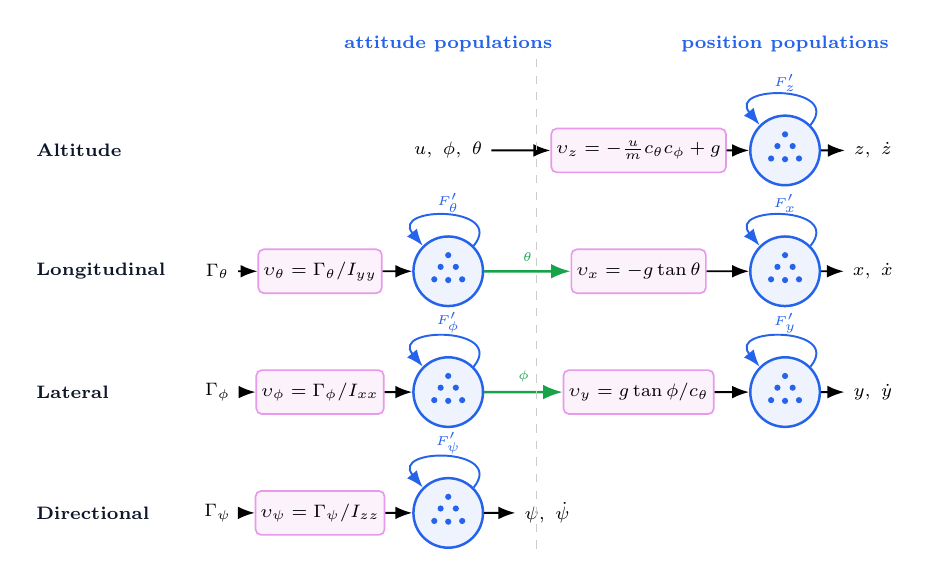
\begin{tikzpicture}[>=Latex, font=\scriptsize, scale=0.93, transform shape,
    pop/.style={draw=primaryblue, circle, line width=0.9pt, minimum size=0.95cm, fill=primaryblue!8, inner sep=0pt},
    ups/.style={draw=morado!80, fill=morado!10, rounded corners=2pt, line width=0.6pt,
                inner sep=2pt, minimum height=0.6cm, align=center},
    lab/.style={font=\scriptsize\bfseries, text=darkslate, anchor=west},
    arr/.style={->, line width=0.7pt}]
  % column headers
  \node[font=\scriptsize\bfseries, text=primaryblue] at (-0.6, 3.95) {attitude populations};
  \node[font=\scriptsize\bfseries, text=primaryblue] at ( 4.0, 3.95) {position populations};
  % ---------------- rows (1.65 cm apart so loops never touch the row above)
  \foreach \y/\n in {2.5/Altitude, 0.85/Longitudinal, -0.8/Lateral, -2.45/Directional}
    \node[lab] at (-6.35, \y) {\n};
  % Altitude: u, phi, theta -> upsilon_z -> z
  \node (inz) at (-0.6, 2.5) {$u,\ \phi,\ \theta$};
  \node[ups] (uz) at (2.0, 2.5) {$\upsilon_z=-\frac{u}{m}c_\theta c_\phi+g$};
  \popn{pz}{(4.0,2.5)}{z}{$F'_z$}
  \node (oz) at (5.2, 2.5) {$z,\ \dot z$};
  \draw[arr] (inz) -- (uz); \draw[arr] (uz) -- (pz); \draw[arr] (pz) -- (oz);
  % Longitudinal: Gamma_theta -> theta -> upsilon_x -> x
  \node (inth) at (-3.75, 0.85) {$\Gamma_\theta$};
  \node[ups] (uth) at (-2.35, 0.85) {$\upsilon_\theta=\Gamma_\theta/I_{yy}$};
  \popn{pth}{(-0.6,0.85)}{\theta}{$F'_\theta$}
  \node[ups] (ux) at (2.0, 0.85) {$\upsilon_x=-g\tan\theta$};
  \popn{px}{(4.0,0.85)}{x}{$F'_x$}
  \node (ox) at (5.2, 0.85) {$x,\ \dot x$};
  \draw[arr] (inth) -- (uth); \draw[arr] (uth) -- (pth);
  \draw[arr, color=forestgreen, line width=0.9pt] (pth) -- node[above, font=\tiny, text=forestgreen]{$\theta$} (ux);
  \draw[arr] (ux) -- (px); \draw[arr] (px) -- (ox);
  % Lateral: Gamma_phi -> phi -> upsilon_y -> y
  \node (inph) at (-3.75, -0.8) {$\Gamma_\phi$};
  \node[ups] (uph) at (-2.35, -0.8) {$\upsilon_\phi=\Gamma_\phi/I_{xx}$};
  \popn{pph}{(-0.6,-0.8)}{\phi}{$F'_\phi$}
  \node[ups] (uy) at (2.0, -0.8) {$\upsilon_y=g\tan\phi/c_\theta$};
  \popn{py}{(4.0,-0.8)}{y}{$F'_y$}
  \node (oy) at (5.2, -0.8) {$y,\ \dot y$};
  \draw[arr] (inph) -- (uph); \draw[arr] (uph) -- (pph);
  \draw[arr, color=forestgreen, line width=0.9pt] (pph) -- node[above, font=\tiny, text=forestgreen]{$\phi$} (uy);
  \draw[arr] (uy) -- (py); \draw[arr] (py) -- (oy);
  % Directional: Gamma_psi -> psi
  \node (inps) at (-3.75, -2.45) {$\Gamma_\psi$};
  \node[ups] (ups) at (-2.35, -2.45) {$\upsilon_\psi=\Gamma_\psi/I_{zz}$};
  \popn{pps}{(-0.6,-2.45)}{\psi}{$F'_\psi$}
  \node (ops) at (0.75, -2.45) {$\psi,\ \dot\psi$};
  \draw[arr] (inps) -- (ups); \draw[arr] (ups) -- (pps); \draw[arr] (pps) -- (ops);
  % separator between attitude and position columns
  \draw[gray!40, dashed] (0.6, 3.75) -- (0.6, -2.95);
\end{tikzpicture}

\vspace{0.1cm}
{\scriptsize Each \textcolor{primaryblue}{circle} is one recurrent LIF population representing
$\chi_\zeta=[\zeta,\ \dot\zeta]^\top$; \textcolor{forestgreen}{green}: attitude drives position.}
\end{frame}

%===================================================================
\section[Control]{Neuromorphic control}

\subsection{Neural integral term}
\begin{frame}{Neural controller: integral term}
\centering
{\small Translational loops are neural \textbf{PID}; attitude loops are neural \textbf{PD}.}

\vspace{0.3cm}
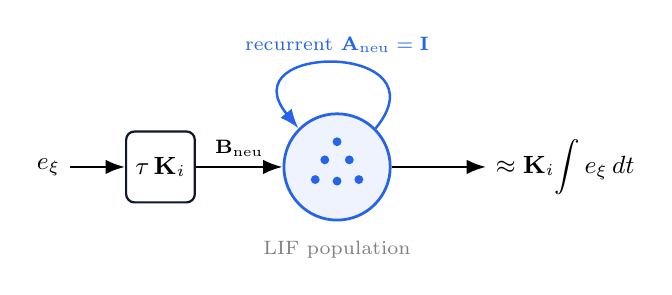
\begin{tikzpicture}[>=Latex, font=\small,
    blk/.style={draw=darkslate, rounded corners=3pt, line width=0.8pt, minimum height=0.9cm, fill=white},
    pop/.style={draw=primaryblue, circle, line width=1pt, minimum size=1.35cm, fill=primaryblue!8}]
  \node (e)  at (0,0) {$e_\xi$};
  \node[blk, right=0.7cm of e] (k) {$\tau\,\mathbf{K}_i$};
  \node[pop, right=1.1cm of k] (p) {};
  \foreach \a/\r in {90/0.32, 210/0.32, 330/0.32, 30/0.18, 150/0.18, 270/0.18}
     \fill[primaryblue] ($(p)+(\a:\r)$) circle (1.6pt);
  \node[right=1.2cm of p] (y) {$\approx \mathbf{K}_i\!\displaystyle\int e_\xi\,dt$};
  \draw[->, line width=0.9pt] (e) -- (k);
  \draw[->, line width=0.9pt] (k) -- node[above, font=\scriptsize]{$\mathbf{B}_{\text{neu}}$} (p);
  \draw[->, line width=0.9pt] (p) -- (y);
  \draw[->, line width=0.9pt, color=primaryblue] (p.north east) .. controls +(0.9,1.1) and +(-0.9,1.1) .. (p.north west)
        node[pos=0.5, above, font=\scriptsize, text=primaryblue] {recurrent $\mathbf{A}_{\text{neu}}=\mathbf{I}$};
  \node[below=0.12cm of p, font=\scriptsize, text=gray] {LIF population};
\end{tikzpicture}

\vspace{0.35cm}
\begin{tcolorbox}[colback=morado!10, colframe=morado!80, width=0.9\linewidth, left=1mm, right=1mm]
\centering\small
$\dot{\mathbf{x}}=\mathbf{A}\mathbf{x}+\mathbf{B}\nu
\ \Rightarrow\ \mathbf{A}_{\text{neu}}=\tau\mathbf{A}+\mathbf{I},\ \ \mathbf{B}_{\text{neu}}=\tau\mathbf{B}$

\vspace{0.1cm}
integrator ($\mathbf{A}=\mathbf{0}$): \ $\mathbf{A}_{\text{neu}}=\mathbf{I},\ \mathbf{B}_{\text{neu}}=\tau\mathbf{K}_i$
\end{tcolorbox}
{\scriptsize The gain $\mathbf{K}_i$ acts on the input, \emph{before} the neural integration.}
\slideref{A. Olivares \emph{et al.}, Neural Comput.\ Appl., 2026.}
\end{frame}

\subsection{From cascade to spiking populations}
\begin{frame}{From the cascade scheme to its spiking realization}
\vspace{-0.1cm}
\centering
\begin{tabular}{@{}c@{\hspace{1.5mm}}c@{}}
\rotatebox{90}{\scriptsize\bfseries\color{darkslate}\ \ Conventional} &
\cascadeTsix{0.64\paperwidth}\\[0.4mm]
 &
{\scriptsize
 \textcolor{magenta}{\rule{0.75em}{0.75em}}\,$z$\quad
 \textcolor{red}{\rule{0.75em}{0.75em}}\,$x$\quad
 \textcolor{green!45!black}{\rule{0.75em}{0.75em}}\,$\theta$\quad
 \textcolor{blue}{\rule{0.75em}{0.75em}}\,$y$\quad
 \textcolor{orange}{\rule{0.75em}{0.75em}}\,$\phi$\quad
 \textcolor{gray}{\rule{0.75em}{0.75em}}\,$\psi$\quad
 \textcolor{teal}{\rule{0.75em}{0.75em}}\,coupling
 \qquad\textcolor{primaryblue}{$\Downarrow$}}\\[0.4mm]
\rotatebox{90}{\scriptsize\bfseries\color{primaryblue}\ \ NEF / Nengo} &
\includegraphics[width=0.53\paperwidth]{images_hexa/Digrama_UAV_dinamyc_ZXTheta-YPhi-3.pdf}
\end{tabular}

\vspace{0.3mm}
{\scriptsize Same colour = same DOF: each PID/PD block $\rightarrow$ error, derivative and $\int$ ensembles.}
\end{frame}

\subsection{Complete architecture}
\begin{frame}{Complete neuromorphic flight-control architecture}
\vspace{-0.3cm}
\makebox[\linewidth][c]{%
\includegraphics[width=\paperwidth,height=0.88\textheight,keepaspectratio]{images_hexa/Digrama_UAV_dinamyc_ZXTheta-YPhi-3.pdf}}

\vspace{-0.05cm}
{\centering\tiny Nonlinear couplings in shared ensembles, e.g.\ $\phi_d=\tan^{-1}(u_y\cos\theta/g)$, $\ \upsilon_y = g\tan\phi/\cos\theta$.\par}
\end{frame}

%===================================================================
\section[Results]{Simulation results}

\subsection{Tracking results}
\begin{frame}{Closed-loop states}
\vspace{-0.15cm}
\centering
{\footnotesize \legdotted{black}\ Ref.\qquad \legsolid{matlabBlue}\ Classic\qquad \legsolid{red}\ SNN/Nengo\par}
\vspace{0.02cm}
\includegraphics[width=\linewidth,height=0.84\textheight,keepaspectratio]{images_hexa/fig01_states_v5_rad.pdf}
\end{frame}

\begin{frame}{Control commands}
\begin{columns}[c,onlytextwidth]
\column{0.80\textwidth}
\centering
\includegraphics[width=\linewidth,height=0.90\textheight,keepaspectratio]{images_hexa/fig02_commands_v5_rads2.pdf}
\column{0.20\textwidth}
\footnotesize
\legsolid{matlabBlue}\\ Classic\\[0.3cm]
\legsolid{red}\\ SNN/Nengo
\end{columns}
\end{frame}

\subsection{Performance indices}
\begin{frame}{Tracking performance over the 60\,s mission}
\begin{table}[h!]
\centering
\small
\begin{tabular}{lcccc}
\toprule
 & \multicolumn{2}{c}{RMSE} & \multicolumn{2}{c}{ISE} \\
\cmidrule(lr){2-3}\cmidrule(lr){4-5}
Variable & Classic & SNN & Classic & SNN \\
\midrule
$x$ [m]        & $0.008$ & $0.032$ & $3.95 \times 10^{-3}$ & $0.0627$ \\
$y$ [m]        & $0.013$ & $0.033$ & $0.0101$ & $0.0660$ \\
$z$ [m]        & $0.019$ & $0.048$ & $0.0213$ & $0.1367$ \\
$\theta$ [rad] & $3.26 \times 10^{-4}$ & $0.005$ & $6.38 \times 10^{-6}$ & $1.71 \times 10^{-3}$ \\
$\phi$ [rad]   & $9.73 \times 10^{-4}$ & $0.012$ & $5.68 \times 10^{-5}$ & $8.67 \times 10^{-3}$ \\
$\psi$ [rad]   & $6.62 \times 10^{-3}$ & $0.009$ & $2.63 \times 10^{-3}$ & $4.61 \times 10^{-3}$ \\
\bottomrule
\end{tabular}
\end{table}
\begin{tcolorbox}[colback = morado!10, colframe = morado!80, title = SNN vs.\ classic correlation $\rho_{\mathrm{SNN,cls}}$]
\centering
$x$: 0.9993 \qquad $y$: 0.9998 \qquad $-z$: 0.9992
\end{tcolorbox}
\end{frame}

%===================================================================
\section[Conclusions]{Conclusions}

\begin{frame}{Conclusions}
\vspace{0.2cm}
\begin{itemize}\setlength\itemsep{10pt}
    \item[\textcolor{forestgreen}{\ding{51}}] \textbf{Dynamics and cascade controller} run as one spiking network (NEF/Nengo).
    \item[\textcolor{forestgreen}{\ding{51}}] It \textbf{reproduces the classic controller}: $\rho>0.999$, position RMSE $<5$\,cm.
    \item[\textcolor{crimsonred}{\ding{55}}] Higher RMSE/ISE than classic: finite ensembles and LIF firing-rate saturation.
    \item[\textcolor{primaryblue}{$\rightarrow$}] \textbf{Next:} full dynamics, disturbances, neuromorphic hardware.
\end{itemize}
\vfill
{\centering\scriptsize Code: \texttt{github.com/esteedeq/UAV\_Nengo}\par}
\end{frame}

\begin{frame}
    \begin{center}
    \textbf{\Huge Thank you for your attention}
    \end{center}
\end{frame}

\end{document}
